\documentclass[10pt,a4paper]{article}
\usepackage[utf8]{inputenc}
\usepackage{mathtools}
\usepackage{amsfonts}
\usepackage{amssymb}
\usepackage{hyperref}
\usepackage{graphicx}
\usepackage[nottoc]{tocbibind}
\newtheorem{theorem}{Theorem}[section]
\newtheorem{lemma}[theorem]{Lemma}
\newtheorem{proof}[theorem]{proof}

\author{Stanley Akor}
\title{Pascal's Triangle Problem}
\begin{document}
\maketitle
\tableofcontents

\newpage
\section{Introduction}
Pascal's triangle is one of the most famous patterns in mathematics, although it may appear to only contain some few patterns, a more detailed study of the triangle opens even more interesting and complicated patterns \ref{triangle}

The study of Pascals triangle began many years before Blaise Pascal was born, the indians and chinesse were among the first people to observe the regular patterns in the triangle, however pascal is attributed for  been the inventor of the triangle because he was the first to organize and compile the information on the triangle so that they actually make sense and are more applicable\cite{siep}

\begin{figure}[h!] \label{triangle}
	\centering
	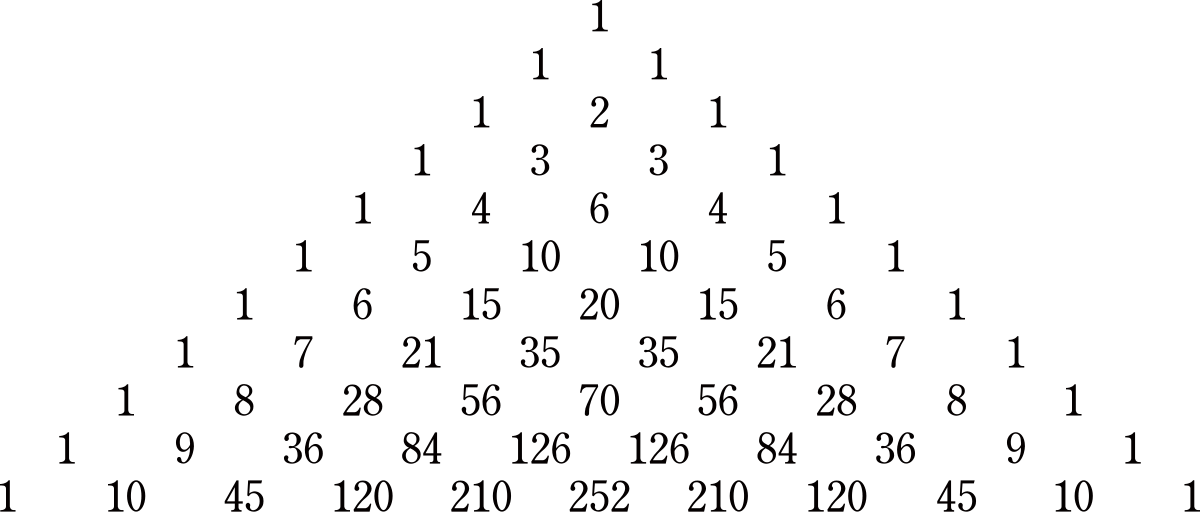
\includegraphics[scale=0.2]{pascal}
	
\caption{Pascal's Triangle}
\end{figure}

\section{Patterns in the Pascal's Triangle}
The numbers in the Pascal's triangle follow some very intriguing patterns, some of which  will be discussed below: 
\subsection{Sum of Rows}
The sum of the numbers in any row of a pascal's triangel equals to $2$ to the power of the number$\left(n\right)$ of that row (that is $2^n$), where the first row is designated as $n=0$ and the second row is is designated as $n=1$ and so on.
\begin{table}[h!]\label{Row}
	\centering
	\begin{tabular}{|c|c|c|}
		\hline 
		Sum of the row	& Row Number$\left(n\right)$  & $2^n$ \\ 
		\hline 
	1=1	& 0 &$2^0$  \\ 
		\hline 
	1+1=2	&1  & $2^1$ \\ 
	\hline
	1+2+1=4	& 2 & $2^1$\\
	\hline 
	1+3+3+1=8	& 3 & $2^2$  \\ 
		\hline 
	1+4+6+4+1=16	& 4 &$2^3$  \\ 
		\hline 
	\end{tabular} 
\caption{Sum of Row in a Pascal's Triangle}
\end{table}

 
we can prove that the sum of the numbers in any row of a pascal's triangle is equal to $2^n$ as shown in Table \ref{Row}, we observe that the next row is twice the row before it, that is Row 3 is twice Row 2, we can prove this by mathematical induction.

It is possible to express the coefficients of a Pascal's Triangle as combinatorial relationship, so we begin our proof by expressing the numbers in any row in combinatorial form.

\newpage
\begin{proof}sum of the numbers in any row of a pascal's triangle is equal to $2^n$
\end{proof}
we know that $C(n,r)=C(n-1,r-1)+C(n-1,r)$ for $1\leq r\leq n-1$. An example of this we would be to let n=3 and r=2 which makes the following statement: $C(3,2)=C(2,1)+C(2,2)$ true!

Our induction assuption is that $n>0$, we have

$C(n-1,0)+C(n-1,1)+C(n-1,2)+..........+C(n-1,n-1)=2^{n-1}$\\
Then lets assume that $C_{n-1,0}+C_{n-1,1}+C_{n-1,2}+....+C_{n-1,n-1}=2^{n-1}$ for $n\geq 1$ which leads us to\\
$C_{n,0}+C_{n,1}+C_{n,2}+....+C_{n,n}=\left(0+C_{n-1,0}\right)+\left
(C_{n-1,0}+C_{n-1,0}\right)+\left(C_{n-1,1}+C_{n-1,2}\right)+.....+\left(C_{n-1,n-1}+0\right)$
$=(0+C_{n-1,0}+C_{n-1,1}+C_{n-1,2}+...+C_{n-1,n-1})+(C_{n-1,0}+C_{n-1,1}+C_{n-1,2}+....+C_{n-1,n-1}+0)$\\
$=2^{n-1}+2^{n-1}=2^{n}$


\subsection{Sierpinski's Triangle}
The Sierpinski's Triangle was discovered by Waclaw Sierpinskin , a Polish mathematiician in 1916, he coloured the odd numbers of the pascals triangle with one colour(Blue) and the even numbers he coloured differently(red)\cite{siep}. Sierpinski was able to describe some of the triangle's interesting properties with his diagram\ref{odds}
\begin{figure}[h!]\label{odds}
\centering
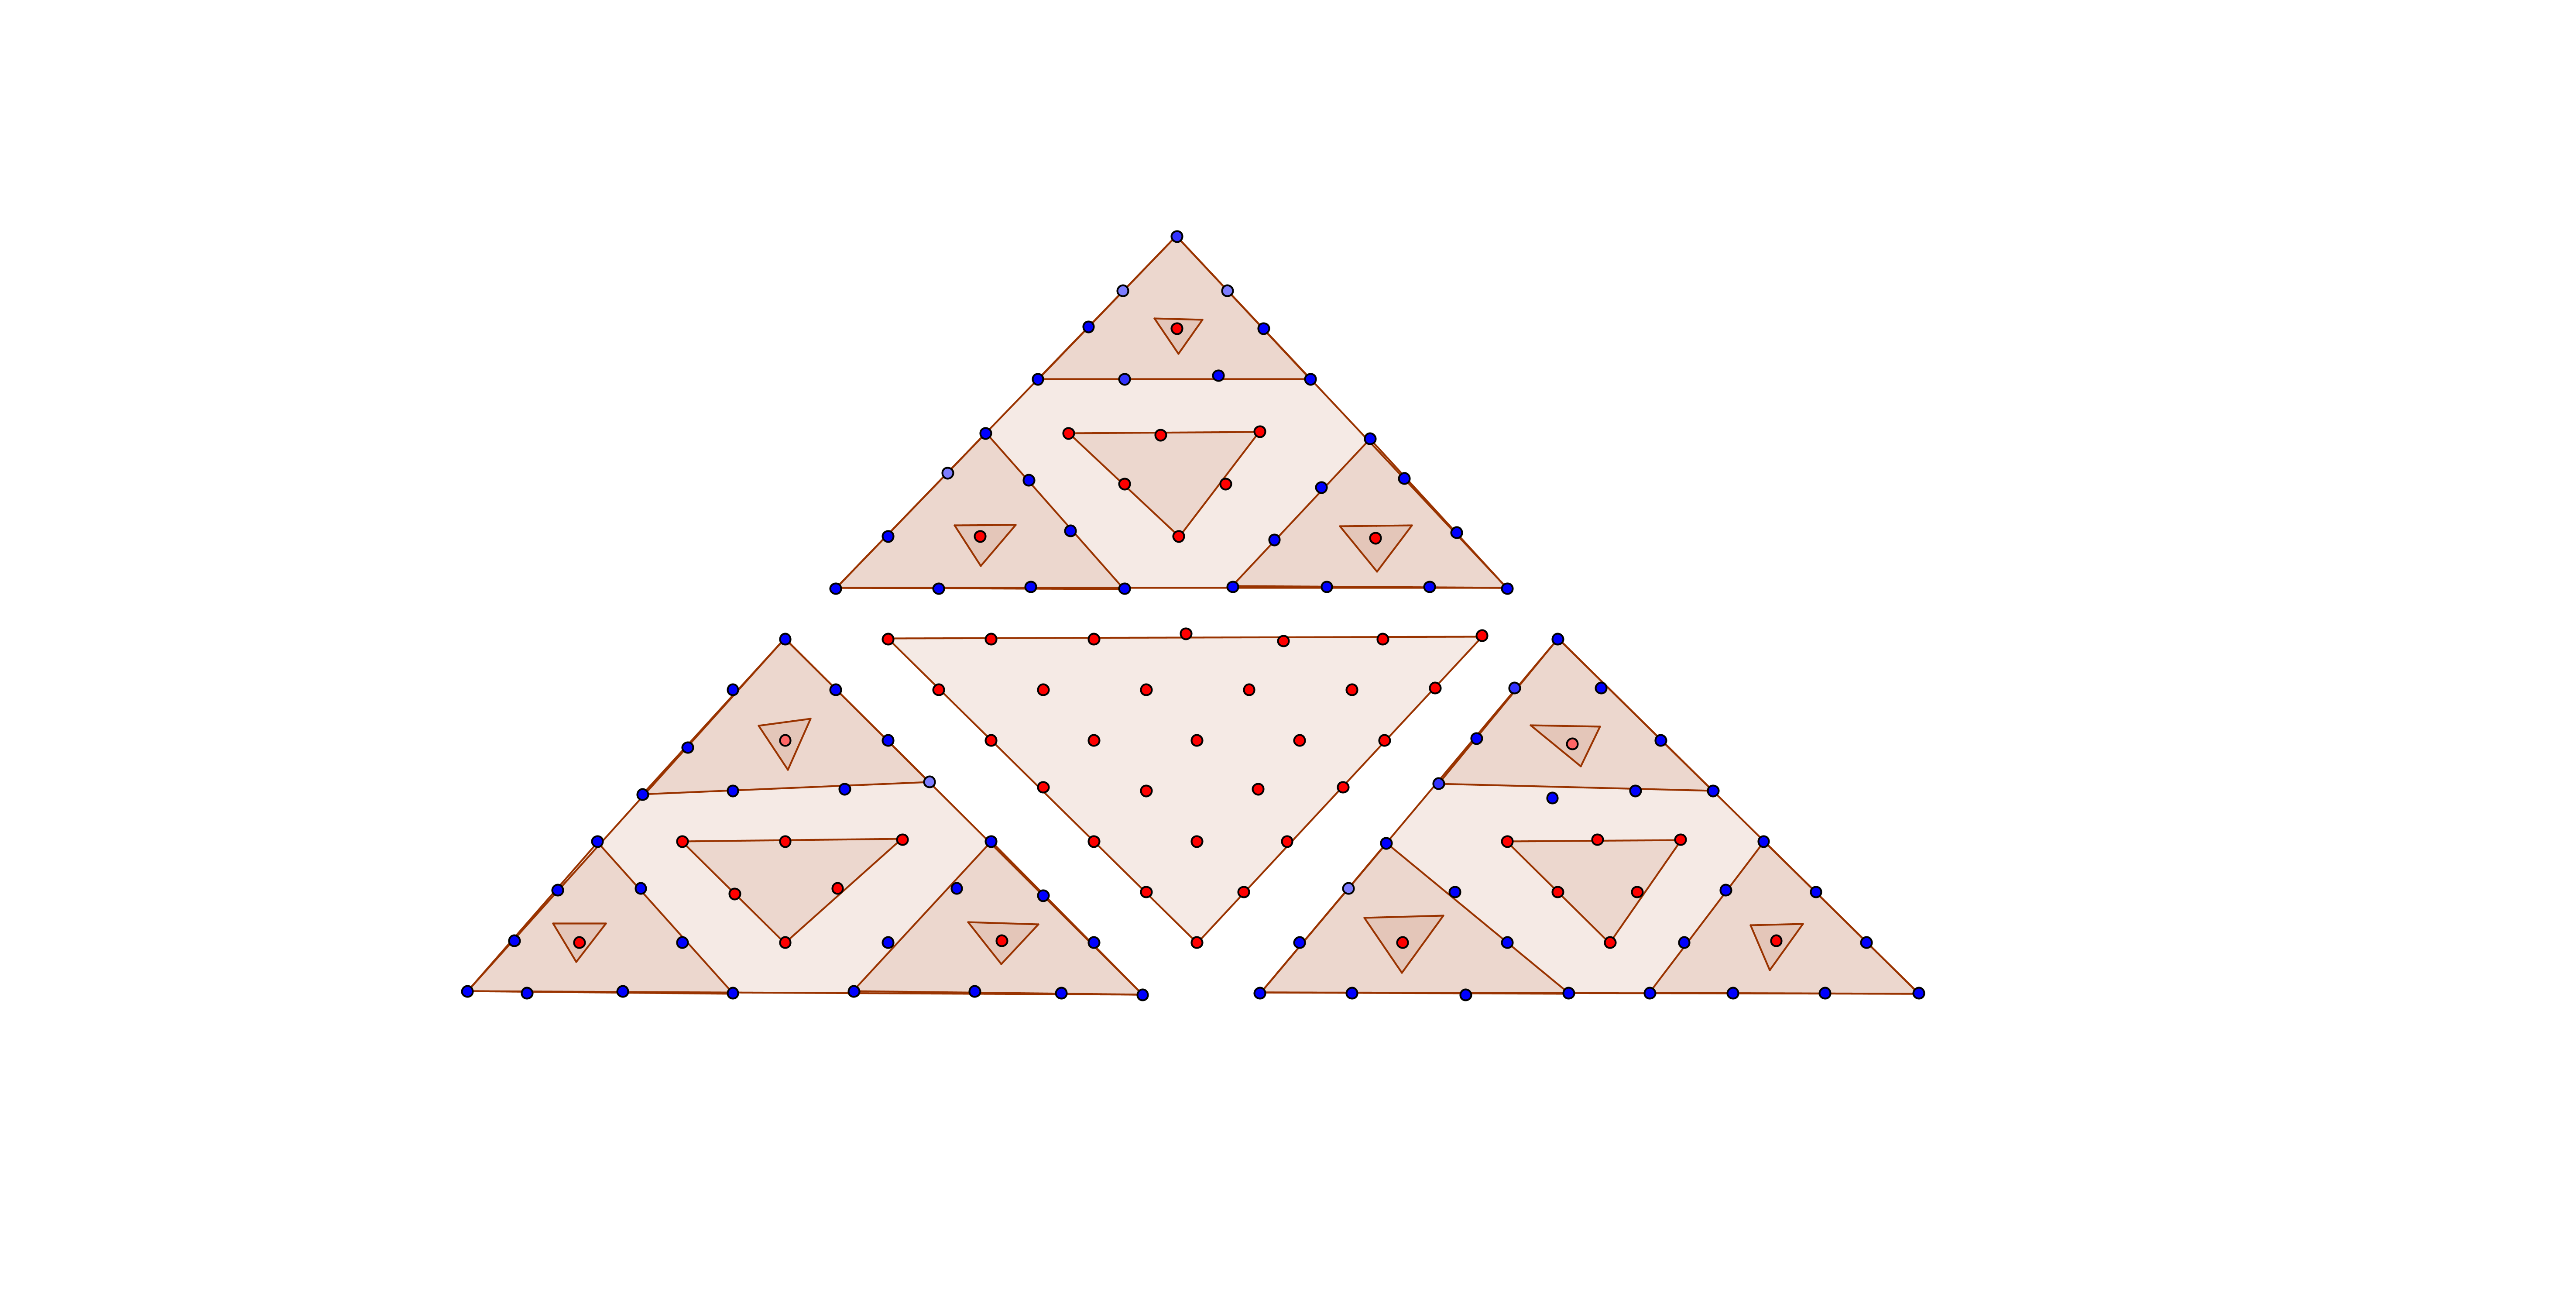
\includegraphics[scale=0.3]{Triangle.png}
	
\caption{The Sierpinski's Triangle}
\end{figure}

\subsubsection{Self-Similarity }
from the sierpinski's triangle we can find a relationship between the big triangle and the smaller triangles inscribed in it, this is the self similarity property,the number of odd digits in the first $2^{nth}$ row is equal to $3^{n}$ where $n$ is the row-number $(n=0,1,2......,n)$ this happens because at every time a new triangle is formed, it always copies 3 times the triangle before it( i.e it copies one to the right,left and above it)\cite{selfs}
\begin{proof}
we want to show that $2^{n}$ equals $3^{n}$
\end{proof}
we want to prove this by INDUCTION.\\
$2^{n}$=$3^{n}$\\
Base Case: when n=0\\
$2^{0}$=$3^{0}$
1=1
so it is True! for n=1\\
Assumption Case:we assusme that it is true for n=k\\
Inductive: for n=k+1\\
$2^{k+1}$\\
at $2^{k+1}$ row, we have 2 copies of $2^{k}$ plus the 1 above, so we have $3\times$$2^{k}$ = 3$\times3^{k}$=$3^{k+1}$

\subsubsection{Odd numbers in each row}
except for the first row where $n=0$ and the number of odd digit is one  (i.e $a(0)=1$),  we can calculate the the number of odd digits in a row by using $a(n)=2\times a(n-2^k)$ where $2^{k}\leq n$ is the greatest $k$ such that $a(n)=2\times a(n-2^k)$. A better generalization of the relation above is the fact that the number of odd elements in any row of the pascal's triangle can be obtained from $2^{sn}$ where $sn$ is the number of 1's in  the binary representation of $n$

\begin{proof}
we want to show that $a(n)=2\times a(n-2^k)$=$2^{Sn}$ 
\end{proof}
$$a(n)=2\times a(n-2^k)=2^{Sn}$$
$$a(0)=1$$
$$n=1\cdot2^{k1}+2^{k2}+2^{k3}+\cdot\cdot\cdot\cdot\cdot+2^{kd}$$   $$ k1>k2>k3\cdot\cdot\cdot\cdot\cdot>kd$$
$$a(n)=2\cdot a(2^{k2}+2^{k3}+2^{kd})$$
$$a(n)=2\cdot2\cdot a(2^{k3}+\cdot\cdot+2^{kd})$$
$$.     .$$
$$.     .$$
$$.     .$$ 
$$.      .$$
$$a(n)=2^{d}\cdot a(0)$$
since $a(0)=1$, $a(n)=2^{d}$ $d=S(n)$,$Sn$ is the binary representation of the row number $(n)$.

\subsubsection{Nature of a number in the Pascal's Triangle}
we can determine the nature of a number in the pascal's triangle (i.e if the number is odd or even) with this formular $\binom{n}{k}$, $n$ is the binary representation of the row number while $k$ is the binary representation of the position of that number in the row, $k$ is odd if in the binary representation of n we have a 1 each time we have 1 in the binary representaion of k, for example, we  want to determine the nature of the 67th element in the 139th row of the pascals triangle
$$\binom{10001011}{01000010}$$ 
Applying the principles stated above, the 67th element will occupy the 66th position because the initial position at each row is 0,  the 67th element in the 139th row will be even (red Coloured)
\section{Conclusion}
The regular patterns in the sequence of numbers  in triangular form is fascinating, as one tends to study these patterns, more intriguing and complicated patterns are formed, the Pascal's Triangle\ref{triangle} is one of many mathematical patterns that is yet to be fully described.
\bibliographystyle{unsrt}
\bibliography{mps.bib}
\end{document}